
\documentclass{article}

\usepackage[ngerman]{babel}                     %for german umlauts
\usepackage[utf8]{inputenc}
\usepackage{subfigure}
\usepackage{float}
%\usepackage[framed,autolinebreaks,useliterate]{mcode}
%\usepackage[bw,framed,autolinebreaks,useliterate]{mcode}
% \usepackage[ansinew]{inputenc}        %for german umlauts

\usepackage{listings}

\usepackage{graphicx}
\usepackage{hyperref}

\usepackage{amssymb}    %for different fonts
\usepackage{amsmath}
% Geht nicht: \usepackage{bbm}
% \usepackage[usenames,dvips]{color} %only way to get it running with pdf:(
% \usepackage[pdftex,usenames,dvipsnames]{color}        % does not work
% \usepackage{color}
\usepackage{verbatim}
\usepackage{polynom}

\setlength{\parindent}{0pt}
\addtolength{\hoffset}{-2cm}
\addtolength{\voffset}{-1cm}
\addtolength{\textheight}{3cm}
\addtolength{\textwidth}{3cm}

\newcommand{\im}{\operatorname{Im}}
\newcommand{\rg}{\operatorname{rg}}
\newcommand{\ggt}{\operatorname{ggT}}

\lstset{ %
  language=Matlab,                % the language of the code
  frame=single,                   % adds a frame around the code
  tabsize=2
}

\begin{document}

\section*{\begin{center} Mustererkennung - Aufgabenblatt 06 \end{center}}
\begin{center}
  André Hacker und Dimitri Schachmann \\
\end{center}


\subsection*{1. PCA}
\subsubsection*{Implementierungs}
Für diese Aufgabe haben wir die Hauptkomponentenanalyse in Matlab
implementiert. Da die Hauptkomponenten schlicht die Eigenvektoren der
Kovarianzmatrix der Daten sind, ist die Funktion ganz einfach:
\begin{lstlisting}
% computes the principal components for the given data
% r = eigenvectors of the covariance matrix
function r = principalComponents(data)
  covarMatrix = cov(data);
  [r eigen_values] = eig(covarMatrix);
end
\end{lstlisting}	
Wenn man nun die Eigenvektoren hat, dann müssen die Daten in die
entsprechende Basis transformiert werden. Dafür haben wir eine
Funktion geschrieben, mit der man zusätlich die Anzahl der Dimensionen
auswählen kann. Es wird angenommmen, dass die längsten Eigenvektoren
ganz rechts in der Matrix sind, also so, wie eig() sie liefert.
\begin{lstlisting}
% trasform data to a new basis, given by eigenspace (eigenvectors)
function r = transformData(eigenspace, data, dim)
  r = (eigenspace(:,end-dim+1:end)'*data')';
end
\end{lstlisting}
Man darf auch nicht vergessen die Daten vor der Analyse zu
standartisieren:
\begin{lstlisting}
% Standardize data by subtracting the mean and deviding by the standard
% deviation
function r = standardize(samples)
  m = mean(samples);
  sd = std(samples);
  for i = 1:size(samples,1)
    samples(i,:) = (samples(i,:) - m) ./ sd;
  end
  r = samples;
end
\end{lstlisting}

Schließlich haben wir das ganze getestet, also die Fisher Diskriminante
mit den ursprünglichen (aber normierten) Daten laufen lassen und dann
noch 16 mal für jeweil 1 bis 16 Dimensionen anhand der PCA.
\begin{lstlisting}
function new_fisher
  % -------
  % TASK 1
  % -------
  % Load the data
  tra = load('pendigits.tra');
  tes = load('pendigits.tes');
  fid = fopen('task1-results.txt','w');
  
  % We standardize the data to adjust for large differences in absolute
  % feature values
  tmp = standardize(tra(:,1:end-1));
  tra = [tmp tra(:,end)];
  tmp = standardize(tes(:,1:end-1));
  tes = [tmp tes(:,end)];

  % here we learn the fisher discriminant using the training data and test
  % it with the test data. We get a matrix of pairwise recognition success
  % rates for the pendigits
  m = test_fisher(tra, tes);
  
  % calculate the avarage success rate
  sr = fisher_success_rate(m);
  fprintf(fid, 'Raw Data Mean Success Rate: %.3f%%\n', 100*sr);

  for dim = 1:16
    save_tra = tra;
    save_tes = tes;

    pcs = principalComponents(tra(:,1:end-1));
    tmp = transformData(pcs, tra(:,1:end-1), dim);
    tra = [tmp tra(:,end)];

    tmp = transformData(pcs, tes(:,1:end-1), dim);
    tes = [tmp tes(:,end)];

    m = test_fisher(tra, tes);
    sr = fisher_success_rate(m);
    fprintf(fid, 'PCA Dimensions: %.0f Mean Success Rate: %.3f%%\n', dim, 100*sr);
    tra = save_tra;
    tes = save_tes;
  end
end
\end{lstlisting} 
Die test\_fisher() Funktion ermittelt die durchschnittliche Erfolgsrate
mit der Fisher Diskriminante.
\begin{lstlisting} 
% compute and test the fisher discriminant
function result = test_fisher(tra, tes)

  result = zeros(10,10);

  for n = 1:9
    for m = n+1:10
      i = n - 1;
      j = m - 1;
      classes = [i j];
      sampel0 = filterByClass(tra, i);
      sampel0 = sampel0(:,1:end-1);
      sampel1 = filterByClass(tra, j);
      sampel1 = sampel1(:,1:end-1);

      testdata = [filterByClass(tes, i); filterByClass(tes, j)];

      % compute multivariate distribution parameters in feature space
      mu0 = mean(sampel0);
      sigma0 = cov(sampel0);
      mu1 = mean(sampel1);
      sigma1 = cov(sampel1);

      a = fisherDiscriminant(mu0, sigma0, mu1, sigma1);

      % compute new mean/variance for 1d distribution on the fisher 
      % discriminant
      psigma0 = a * sigma0 * a';
      psigma1 = a * sigma1 * a';
      pmu0 = project(mu0, a);
      pmu1 = project(mu1, a);
    
      % test with test data
      projection = project(testdata(:,1:end-1), a);

      % compute the propabilties for each test sample and the two classes.
      P = [gaussDensity(pmu0, psigma0, projection) ...
           gaussDensity(pmu1, psigma1, projection) ];

      [maxValue maxIndex] = max(P,[],2);
      
      % contains the predicted classes
      class = classes(maxIndex)';

      % computes the success rate of prediction
      success = analyze([class testdata(:,end)]);
      result(n,m) = success;
    end
  end
end
\end{lstlisting} 
Die Fisher Diskriminate wird gewohnt wie folgt berechnet:
\begin{lstlisting} 
function direction = fisherDiscriminant( mean1, covar1, mean2, covar2 )
  u = (mean1 - mean2) / (covar1 + covar2);
  direction = u / norm(u);
end
\end{lstlisting} 
Der Vollständigkeit halber sind im folgenden weitere Hilfsfunktionen zu sehen:
\begin{lstlisting} 
function p = gaussDensity(mu, sigma, data)
  normalize = 1 / (sqrt(2*pi) * sigma);
  p = zeros(size(data,1), 1);
  for i=1:size(data,1)
    p(i) = normalize * exp( -(data(i)-mu)^2 / (sigma^2) );
  end

end

function r = filterByClass(samples, c)
  r = samples(ismember(samples(:,end),c),:);
end

function p = project(x, a)
  if (size(x,1)>1)
    p = dot(x, repmat(a, size(x,1),1), 2);
  else
    p = dot(x,a);
  end
end

function success = analyze(isVsShould)

  hit = 0;
  miss = 0;

  misses = zeros(10,10);
  hits = zeros(1,10);

  for k = 1:size(isVsShould, 1)
    if isVsShould(k,1) == isVsShould(k,2)
      hit = hit +1;
      hits(isVsShould(k,2)+1) = hits(isVsShould(k,2)+1) + 1;
    else
      miss = miss + 1;
      misses(isVsShould(k,1)+1,isVsShould(k,2)+1) = misses(isVsShould(k,1)+1,isVsShould(k,2)+1) + 1;

    end;
  end;

  success = 1-(miss/(hit+miss));
end

function r = fisher_success_rate(s)
  r = 0;
  for n = 1:9
    for m = n+1:10
      r = r + s(n,m);
    end
  end
  r = r / (9*10/2);
end
\end{lstlisting} 
\subsubsection*{Auswertung}
Wir haben festgestellt, dass in diesem Fall die
Hauptkomponentenanalyse die, schon ausgezeichneten, Erkennungsraten
nicht deutlich verbessert, aber bei geringerem Rechenaufwand auch nicht
viel verschlechtert. Die durchschnittlichen Erkennungsraten sind im
folgenden zu sehen:
\begin{samepage}
\verbatiminput{task1-results.txt}
\end{samepage}
Es ist gut zu sehen, dass die Erkennungsrate für PCA mit allen
Dimensionen die gleiche ist, wie die ohne PCA. Das ist verständlich,
denn in diesem Fall unterscheiden sich die Daten nur in der Rotation.

Im folgenden noch die paarweisen Erfolgsraten. Erstmal ohne PCA:
	\begin{table}[H]
	    \begin{tabular}{|l|l|l|l|l|l|l|l|l|l|l|}
	        \hline
                & 1      & 2      & 3      & 4      & 5      & 6      & 7      & 8      & 9      \\ \hline
         0&    0.9807 &    0.9876&    0.9986&    0.9986&    0.9670&    0.9957&    0.9835&    0.9342&    0.9771\\
         1&         0&    0.9643&    0.9914&    0.9945&    0.9957&    0.9971&    0.9313&    1.0000&    0.9043\\
         2&         0&         0&    0.9971&    0.9973&    0.9785&    1.0000&    0.9945&    0.9971&    0.9986\\
         3&         0&         0&         0&    0.9986&    0.9896&    0.9970&    0.9771&    0.9970&    0.9866\\
         4&         0&         0&         0&         0&    1.0000&    0.9900&    0.9766&    0.9971&    0.9971\\
         5&         0&         0&         0&         0&         0&    0.9940&    0.9571&    0.9642&    0.9642\\
         6&         0&         0&         0&         0&         0&         0&    0.9914&    0.9926&    0.9985\\
         7&         0&         0&         0&         0&         0&         0&         0&    0.9971&    0.9557\\
         8&         0&         0&         0&         0&         0&         0&         0&         0&    0.9970\\
	        \hline
	    \end{tabular}
	\end{table}

Und jetzt mit PCA und 10 Dimensionen:
	\begin{table}[H]
	    \begin{tabular}{|l|l|l|l|l|l|l|l|l|l|l|}
	        \hline
          &1         &2         &3         &4         &5         &6         &7         &8         &9 \\ \hline
         0&    0.9807&    0.9986&    0.9986&    0.9959&    0.9642&    0.9900&    0.9807&    0.9285&    0.9742\\ 
         1&         0&    0.9245&    0.9757&    0.9959&    0.9957&    0.9914&    0.9327&    0.9786&    0.8757\\ 
         2&         0&         0&    1.0000&    1.0000&    0.9943&    1.0000&    0.9821&    0.9929&    0.9986\\ 
         3&         0&         0&         0&    0.9957&    0.9836&    0.9970&    0.9714&    0.9955&    0.9762\\ 
         4&         0&         0&         0&         0&    0.9814&    0.9957&    0.9753&    0.9900&    0.9971\\ 
         5&         0&         0&         0&         0&         0&    0.9791&    0.9742&    0.9419&    0.9508\\ 
         6&         0&         0&         0&         0&         0&         0&    1.0000&    0.9911&    0.9896\\ 
         7&         0&         0&         0&         0&         0&         0&         0&    0.9743&    0.9529\\ 
         8&         0&         0&         0&         0&         0&         0&         0&         0&    0.9955\\ 
	        \hline
	    \end{tabular}
	\end{table}
        Hier sieht man, dass mit weniger Dimensionen die
        Erkennungsrate sogar etwas besser sein kann, wie z.B. mit den
        Ziffern 3 und 2.\\
        
        \textbf{Visualisierung}:
        Wir haben angenommen dass die Visualisierung wie in der Mail von Therese vorgeschlagen zu interpretieren ist.\\
        Das heißt wir berechnen die Hauptachsen für alle Trainingsdaten, transformieren die Trainingsdaten in diese neue Basis
        und zeigen das Ergebnis als Zahl an. Wir haben Beispielhaft die ersten 8 Beispiele aus den Trainingsdaten visualisiert.
        
		\begin{lstlisting}
  % Visualize some digits
  pc = principalComponents(tra(:,1:end-1));
  tmp = transformData(pc, tra(:,1:end-1), 16);
  for i=1:10
    h = figure('NumberTitle','on');
    hold on;
    plot( tmp(i,1:2:end-1), tmp(i,2:2:end) );
    title(['Training item ' mat2str(i) ' Digit ' mat2str(tra(i,end))], 'FontSize', 30);
    print(h,'-deps',['task1-transformed-digit-' mat2str(i) '.eps']);
  end
		\end{lstlisting} 
		Hier die transformierten ersten 8 Exemplare aus den Trainingsdaten
		
	\begin{figure}[H]
	  \begin{subfigure}
	    \centering
	    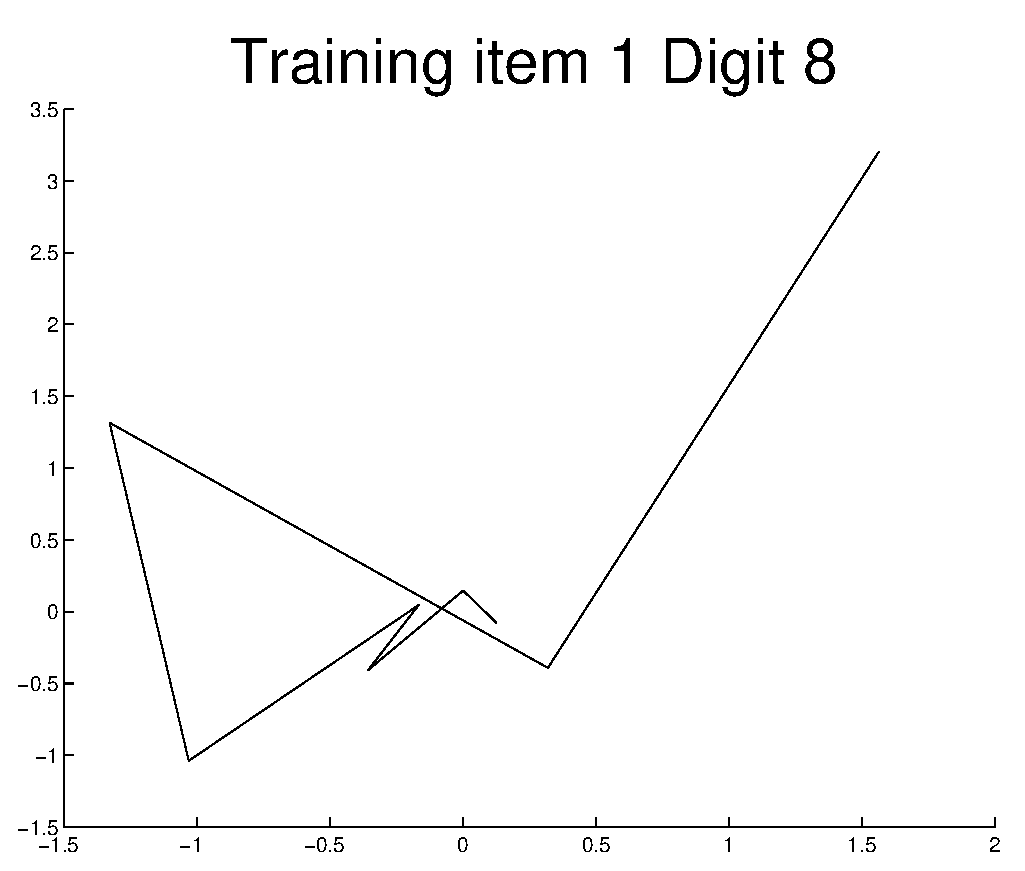
\includegraphics[scale=0.4]{task1-transformed-digit-1.eps}
	  \end{subfigure}
	  \begin{subfigure}
	    \centering
	    \includegraphics[scale=0.4]{task1-transformed-digit-2.eps}
	  \end{subfigure}
	\end{figure}
	\begin{figure}[H]
	  \begin{subfigure}
	    \centering
	    \includegraphics[scale=0.4]{task1-transformed-digit-3.eps}
	  \end{subfigure}
	  \begin{subfigure}
	    \centering
	    \includegraphics[scale=0.4]{task1-transformed-digit-4.eps}
	  \end{subfigure}
	\end{figure}
	\begin{figure}[H]
	  \begin{subfigure}
	    \centering
	    \includegraphics[scale=0.4]{task1-transformed-digit-5.eps}
	  \end{subfigure}
	  \begin{subfigure}
	    \centering
	    \includegraphics[scale=0.4]{task1-transformed-digit-6.eps}
	  \end{subfigure}
	\end{figure}
	\begin{figure}[H]
	  \begin{subfigure}
	    \centering
	    \includegraphics[scale=0.4]{task1-transformed-digit-7.eps}
	  \end{subfigure}
	  \begin{subfigure}
	    \centering
	    \includegraphics[scale=0.4]{task1-transformed-digit-8.eps}
	  \end{subfigure}
	\end{figure}
        
\subsection*{2. Perceptron}

\subsubsection*{a) Daten generieren}
	Die Klassifizierung erfolgt aufgrund eines vorgegebenen Gewichts, und somit sind die Daten linear trennbar. Folgender Code erzeugt die Daten:
	
	\begin{lstlisting}
	% Create linear separable labled data with bias
	% X = random items
	% y = label, based on w
	% w = random weigth
	% dim = dimension
	function [X, y, w] = linSepData(rows, dim)
	  X = [ones(rows,1) rand(rows, dim-1)*2-1];
	  w = rand(1, dim)*2-1;
	  y = perceptronPredict(X,w);
	end
	
	% Predict using the weight w with threshold 0
	function y = perceptronPredict(X, w)
	  y = X*w';
	  y(y>=0)=1;
	  y(y<0)=0;
	end
	\end{lstlisting}
	
	
\subsubsection*{b) Lernen}
	In unserer Lösung wird in jeder Iteration zuerst geprüft, ob die aktuelle Gewichtung bereits fehlerfrei trennt. Falls nicht, wird \textbf{zufällig} einer der falsch zugeordneten Vektoren ausgewählt und anhand von diesem werden die Gewichte angepasst.\\
	
	Folgender Code löst Aufgabe 2:
	\begin{lstlisting}
  % -------
  % TASK 2 Perceptron
  % -------
  items = 1000;
  fid = fopen('task2-results.txt','w');

  % a) Create test data
  [X, y, w] = linSepData(items, 4);
  
  % b) Learn using Perceptron
  [w2, steps, E] = perceptron(X, y, 10000);
  plotPerceptronError(E, 'task2-perceptron');

  % Compare original and learned weight
  fprintf(fid, 'Generated %d items\n', items );
  fprintf(fid, 'Required iterations: %d\n', steps);
  fprintf(fid, 'Original weigth: %s\n', mat2str(w,3) );
  fprintf(fid, 'Learned weigth: %s\n', mat2str(w2,3) );
  fclose(fid);
	\end{lstlisting}
	
	Hier die relevanten Funktionen:
	\begin{lstlisting}
% Learn the weights using PLA
% w = learned weight
% steps = number of needed steps
% E = Error for each iteration
function [w steps E] = perceptron(X, y, maxSteps)
  w = rand(1, size(X,2))*2-1;
  E = [[1:maxSteps]', zeros(maxSteps,1)]; % Track error for each iteration
  for i=1:maxSteps
    % Already finished?
    wrongIds = getWrongClassified(X, y, w);
    E(i,2) = size(wrongIds,1);
    if size(wrongIds, 1) == 0
      break
    end

    % Weight improvement (for any wrong classified)
    id = wrongIds(randi(size(wrongIds,1)),:);
    if y(id) == 1 % false negative (should be 1)
      w = w + X(id, :);
    else  % false positive
      w = w - X(id, :);
    end
  end
  steps = i;
  E = E(1:i,:);
end

% Predict using the weight w with threshold 0
function y = perceptronPredict(X, w)
  y = X*w';
  y(y>=0)=1;
  y(y<0)=0;
end

% Classify and test whether we all is classified correctly
% if not, we return the indicies of all wrong item
function wrongIds = getWrongClassified(X, y, w)
  % Predict
  p = perceptronPredict(X,w);
  diff = y - p;

  % Get wrong
  % any selects the rows different from 0
  wrongIds= [1:size(X,1)]';
  wrongIds = wrongIds(any(diff,2));
end

% Plot Perceptron Error rate
function plotPerceptronError(E, name)
  h = figure();
  hold on;
  xlabel('Iteration', 'FontSize', 15);
  ylabel('Wrong classified', 'FontSize', 15);
  plot(E(:,1),E(:,2));
  print(h,'-deps',[name '.eps']);
end
	\end{lstlisting}
	
	Wir erhalten folgende Ausgabe:
	\verbatiminput{task2-results.txt}
	Wir sehen, dass sowohl die Vorzeichen als auch das Verhältnis der Koeffizienten im Wesentlichen übereinstimmen. Da wir einen reellen Raum haben gibt es sehr viele (unendlich viele) Lösungen.\\
	
	Im folgenden ein Plot der Fehlerrate (hier Anzahl falsch klassifizierter Werte) für jede Iteration. Dieses schwankt natürlich stark in Abhängigkeit von den initialen Gewichten:
	\begin{figure}[H]
	  \begin{subfigure}
	    \centering
	    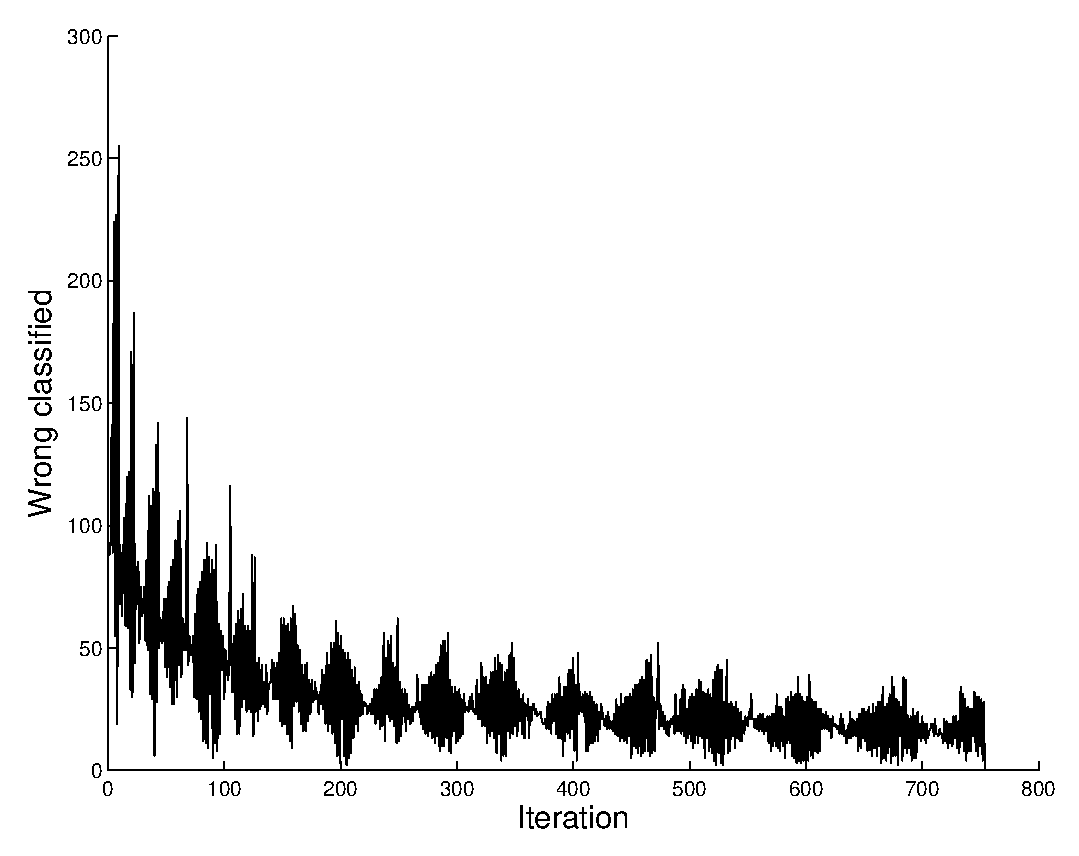
\includegraphics[scale=0.75]{task2-perceptron.eps}
	  \end{subfigure}
	\end{figure}

\subsection*{3. Perceptron Kantenerkennung}
	
	\subsubsection*{a) Daten generieren}
	
	Die möglichen Inputs sind genau durch die möglichen 9-stelligen binären Zahlen beschrieben.\\
	Durch Nachdenken erhält man die Gewichte $w = (-1, 1, 1, 1, 1, -10, 1, 1, 1, 1)$ für eine korrekte Klassifizierung.\\
	
	Folgender Code löst Aufgabe 3 a):
	\begin{lstlisting}
	% Generate data for task3
	function [X, y, w] = task3ImageData()
	  X = dec2bin(0:2^9-1)-'0';
	  X = [ones(size(X,1),1) X];
	  % 0=black, 1=white, mid must be black for edge
	  % This is a working weighting:
	  w = [-1 1 1 1 1 -10 1 1 1 1];
	  y = perceptronPredict(X,w);
	end
	\end{lstlisting}
	
	\subsubsection*{b) Lernen und Testen}
	
	Analog zu 2 werden die Gewichte gelernt.\\
	Anschließend wird jeder Pixel eines Bildes (außer am Rand) mit der gelernten Schwellenwertfunktion klassifiziert (Kante oder nicht). 
        Dabei wird jeder Pixel einzeln anhand seiner Umgebung klassifiziert, und nicht etwa alle 9 in einem 3 $\times$ 3 Feld.
	\begin{lstlisting}
  % -------
  % TASK 3
  % -------
  % a) Create correctly classified data
  [X, y, w] = task3ImageData();

  % b) Learn weights
  [w2, steps, E] = perceptron(X, y, 10000);
  plotPerceptronError(E, 'task3-perceptron');
  fid = fopen('task3a-results.txt','w');
  fprintf(fid, 'Required iterations: %d\n', steps);
  fprintf(fid, 'Original weigth: %s\n', mat2str(w,3) );
  fprintf(fid, 'Learned weigth: %s\n', mat2str(w2,3) );
  fclose(fid);

  detectContour(w2);
  
  ...
  
	% Detect contours in a sample image
	function detectContour(w)
	  % Circle (from Barbara Haupt)
	  [xs,ys]=meshgrid(-100:100);
	  I=zeros(size(xs));
	  I(sqrt(xs.^2+ys.^2)<(0.3*size(xs,1)))=1;
	  h = figure;
	  imagesc(I); colormap('gray'); axis equal off;
	  print(h,'-deps',['task3b-original.eps']);
	
	  % Detect contours
	  h = figure;
	  X = zeros(size(xs));
	  for i=2:size(xs,1)-1
	    for j=2:size(xs,1)-1
	      x = [1, ...
	        I(i-1,j-1), ...
	        I(i-1,j), ...
	        I(i-1,j+1), ...
	        I(i,j-1), ...
	        I(i,j), ...
	        I(i,j+1), ...
	        I(i+1,j-1), ...
	        I(i+1,j), ...
	        I(i+1,j+1)];
	      X(i,j) = perceptronPredict(x, w);
	    end
	  end
	  imagesc(X); colormap('gray'); axis equal off;
	  print(h,'-deps',['task3b-contours.eps']);
	end
	\end{lstlisting}
	
	Wir erhalten folgende Ausgabe:
	\verbatiminput{task3a-results.txt}
	Erneut sehen wir, dass die Vorzeichen und das Verhältnis der Koeffizienten mit unserer naiv gewählten Variante übereinstimmen.\\
	
	Originalbild:
	\begin{figure}[H]
	  \begin{subfigure}
	    \centering
	    
\includegraphics[scale=0.75]{task3b-original.eps}
	  \end{subfigure}
	\end{figure}
	
	Bild der Kanten:
	\begin{figure}[H]
	  \begin{subfigure}
	    \centering
	    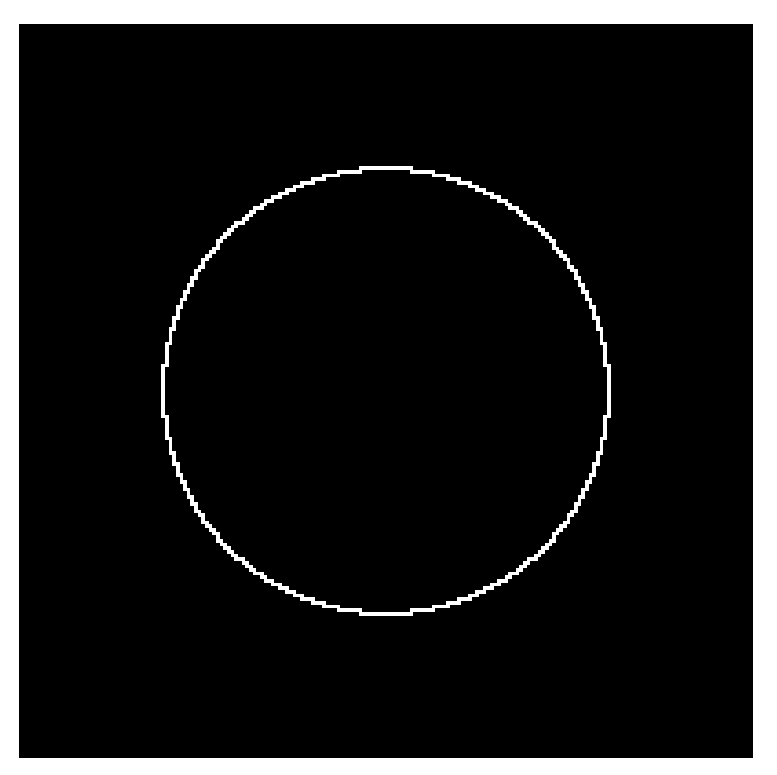
\includegraphics[scale=0.75]{task3b-contours.eps}
	  \end{subfigure}
	\end{figure}
	
	Fehlerrate beim Lernen der Gewichte:
	\begin{figure}[H]
	  \begin{subfigure}
	    \centering
	    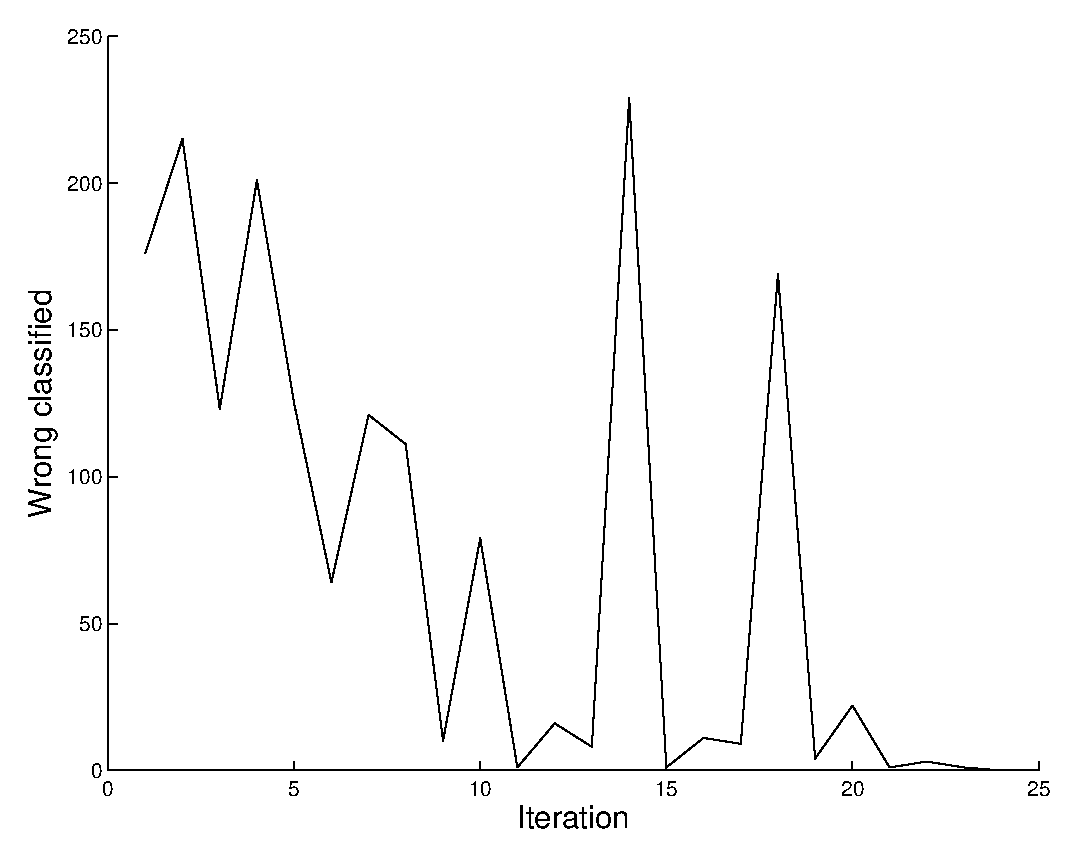
\includegraphics[scale=0.75]{task3-perceptron.eps}
	  \end{subfigure}
	\end{figure}
	
	
\end{document}